\section{Resultados}

\subsection{Estação de Medidas}

\subsubsection{Leitura dos sensores}

\subsubsection{Transmissão das leituras - Advertising}

Para verificar os pacotes transmitidos pela estação de medidas utilizou-se o
aplicativo nRF Connect versão 4.19.1 disponível para smartphones Android. Com
este aplicativo é possível listar os dispositivos bluetooth presentes nas
proximidades, além de ser possível verificar os dados dentro dos pacotes. O
aplicativo também permite o estabelecer conexões com o dispositivo para acessar
os serviços e características.

Na tela inicial do aplicativo é possível ver a estação de medidas listada como
dispositivo próximo com o nome \dblquote{UFABC001} bem como seu MAC Address,
como mostra a figura \ref{fig:nrfconnect_root}. Logo a frente do nome do
dispositivo há a marcação \dblquote{(Nordic)}, que se deve ao fato do
dispositivo utilizar pacotes codificados como Manufacturer Specific Data.


\begin{center}
	\centering 
	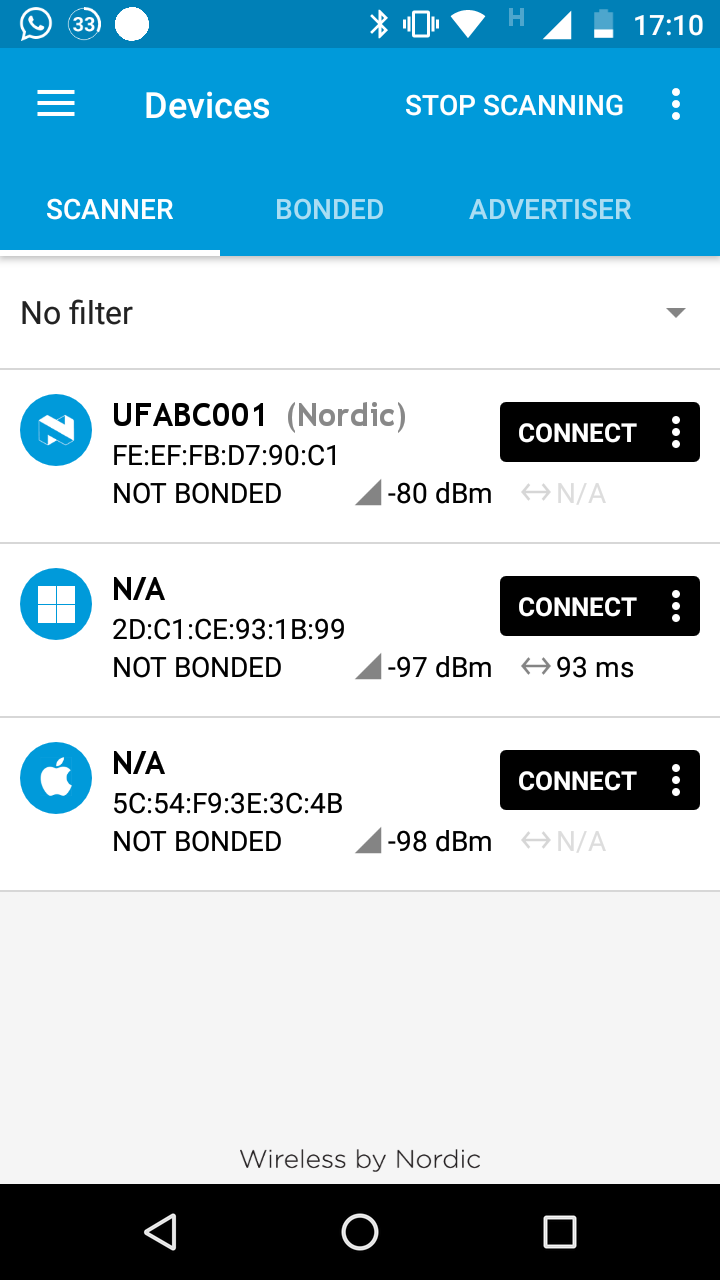
\includegraphics[width=0.4\linewidth]{nrf_connect_adv.png}
	\captionof{figure}{Lista dos dispositivos detectados pelo aplicativo nRF
	Connect}
	\label{fig:nrfconnect_root}
\end{center} 

Ao selecionar o dispositivo, observam-se mais informações sobre os pacotes
recebidos por aquele dispositivo. Na figura \ref{fig:nrfconnect_device} é
possível ver as informações referentes ao pacote decodificadas, como o
\dblquote{Device Type}, indicando que esta estação de medidas opera somente com
o BLE e não com o bluetooth clássico, as flags de pacote indicando que o pacote
é detectável por qualquer dispositivo. O pacote também mostra o Complete Local
Name, que é transmitido nos pacotes de Scan Response como previsto no projeto, e
um conjunto de bytes referentes ao Manufacturer Specific Data, e nesse pacote se
encontram as leituras dos sensores.

\begin{center}
	\centering 
	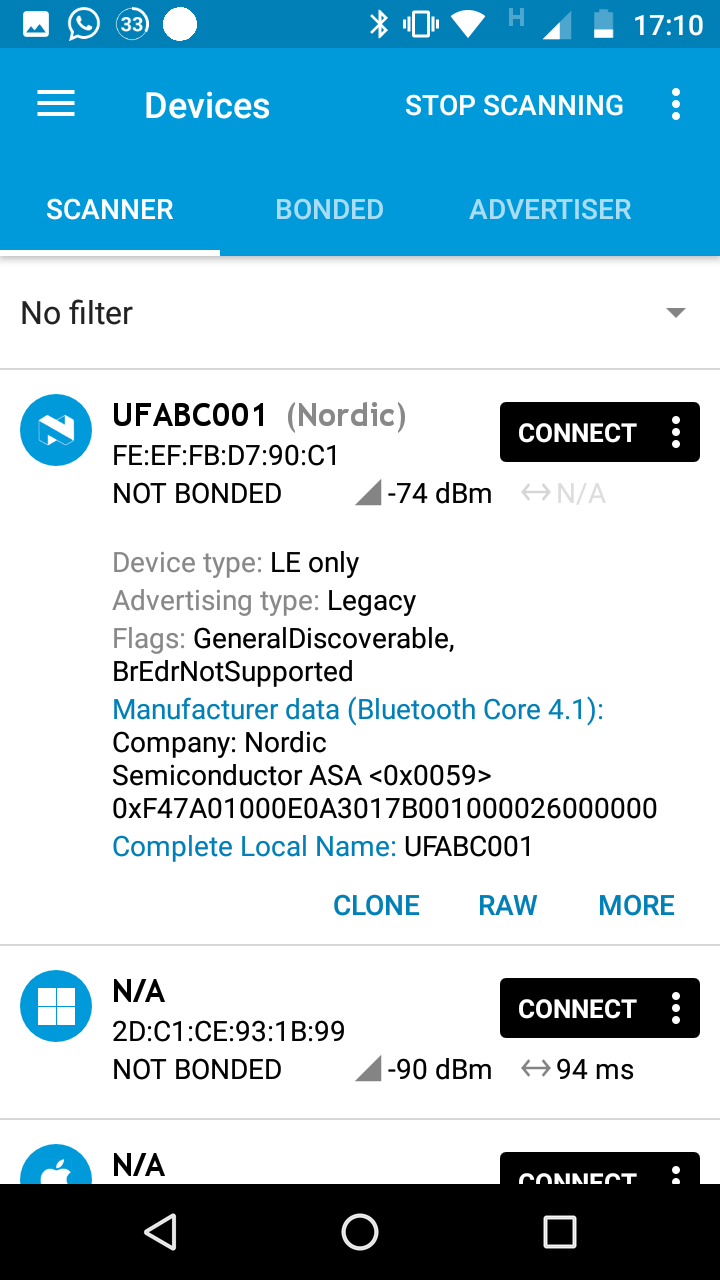
\includegraphics[width=0.4\linewidth]{nrf_connect_device.png}
	\captionof{figure}{Informações do pacote de advertising recebido}
	\label{fig:nrfconnect_device}
\end{center} 

Encaixando o pacote de dados no campo Manufacturer Specific Data da figura
\ref{fig:nrfconnect_device} na estrutura de dados descrita no código fonte
\ref{lst:struct_adv} se obtém os dados decodificados dos sensores conforme o
que é feito na tabela \ref{tab:decoded_adv}. Os dados recebidos pelo bluetooth
seguem o padrão Big Endian (abreviado como \dblquote{b.e.} na tabela) deixando
os bytes mais significativos na última posição do vetor, enquanto a
interpretação dos dados segue o padrão Little Endian (abreviado como
\dblquote{l.e.} na tabela) trabalha com os bytes menos significativos na última
posição do vetor.

\begin{centering}
\vfill
\footnotesize
\begin{tabular}{| c | c | c | c | c | c |}

\hline 
\textbf{Variável} & \textbf{pressure} & \textbf{temperature} & \textbf{humidity} & \textbf{visible lux} & \textbf{infrared lux} \\ \hline 
Tipo & uint32 & int16 & uint16 & uint32 & uint32 \\ \hline
Tamanho & 4 bytes & 2 bytes & 2 bytes & 4 bytes & 4 bytes \\ \hline
Byte code (b.e.)& 0xF47A0100 & 0x0E0A & 0x3017 & 0xB0010000 & 0x26000000 \\ \hline
Byte code (l.e.)& 0x00017AF4 & 0x0A0E & 0x1730 & 000001B0 & 0x00000026 \\ \hline
Valor decimal & 97012 &  2574 & 5936 & 432 & 38 \\ \hline
\end{tabular}
% \normalsize 
\label{tab:decoded_adv}
\captionof{table}{Pacote de dados dos sensores decodificado}
\end{centering}

Tratando as unidades dos dados da tabela, os valores lidos dos sensores são:
\begin{itemize}
  \item Pressão: 97012 Pa
  \item Temperatura: $25.74\,^{\circ}{\rm C}$
  \item Umidade do ar: 59.36 \%RH
  \item Luminosidade Visível: 432 LUX
  \item Luminosidade Infravermelha: 38 LUX
\end{itemize}

\subsubsection{Serviços Bluetooth}

Ainda utilizando aplicativo nRF Connect, são testados os serviços Bluetooth
presentes na estação de medidas.

Para o teste dos serviços, é necessário realizar a conexão através do botão
\dblquote{Connect}, que automaticamente abre uma aba referente ao dispositivo.
Ao completar o processo de conexão, são listados todos os serviços do
dispositivo, sendo os serviços padronizados pelo Bluetooth listados com seus
nomes e os serviços customizados (como os deste trabalho) possuem o nome
\dblquote{Unknown Service}, como mostra a figura \ref{fig:svc-view}.

É possível ver também que no campo UUID está presente a sequência de bytes
definida no código fonte \ref{lst:base_uuid} em conjunto com os identificadores
de 2 bytes presentes nos códigos fonte \ref{lst:apss_uuid}, \ref{lst:thss_uuid}
e \ref{lst:lss_uuid}, que ocupam as posições 2 e 3 da sequência de bytes,

\begin{center}
	\centering 
	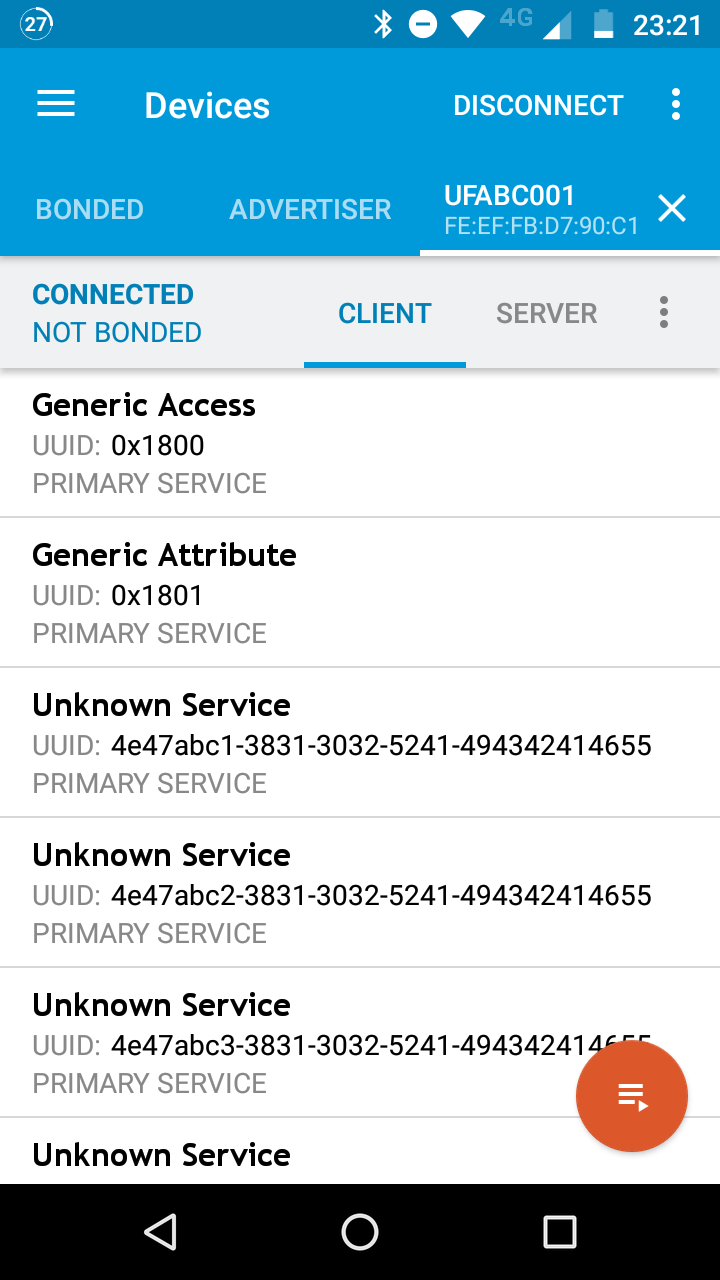
\includegraphics[width=0.4\linewidth]{svc-view.png}
	\captionof{figure}{Lista de serviços Bluetooth presentes no dispositivo}
	\label{fig:svc-view}
\end{center} 


Ao extender o serviço com UUID 0xABC1 (APSS), são listadas as características do
serviço, como mostra a figura \ref{fig:svc-char-view}. As características com
identificação. O UUID de cada característica é localizado nos bytes 2 e 3. As
características com UUID 0x0A00, 0x0A01 e 0x0A02 (as de configuração) são
mostradas com as propriedades \dblquote{READ} e \dblquote{WRITE}. Já a
característica mostrada com UUID 0x0A03 possui as propriedades \dblquote{READ} e
\dblquote{NOTIFY}, de acordo com o projeto do serviço.


Realizando a leitura de todas as características, observa-se as configurações do
sensor de pressão bem como a ultima leitura realizada como visto na figura
\ref{fig:svc-char-read}. Ao ativar a notificação, as leituras de pressão são
atualizadas automaticamente.


\begin{center}
	\centering 
	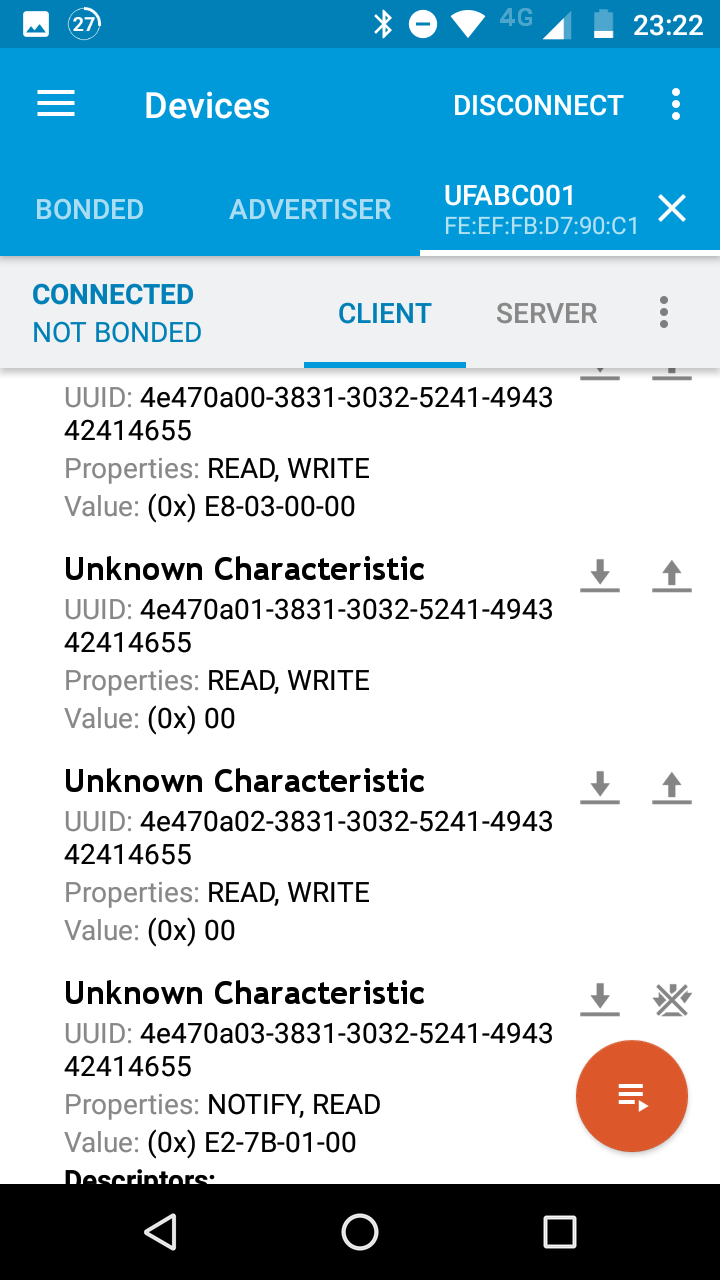
\includegraphics[width=0.4\linewidth]{svc-char-read.png}
	\captionof{figure}{Valores lidos das características}
	\label{fig:svc-char-read}
\end{center} 

\subsection{Gateway Bluetooth - Internet}

\subsubsection{Bluetooth Observer}
 
%TODO MAC, RSSI
O primeiro teste realizado sobre o funcionamento do Bluetooth Observer foi a
obtenção de pacotes com envio das informações recebidas através da porta serial
do microcontrolador, mostrando os dados: endereço MAC, RSSI do sinal, o tamanho
do pacote recebido e os dados do pacote. A figura \ref{fig:adv_list} mostra as
mensagens recebidas através de um terminal serial.

\begin{center}
	\centering 
	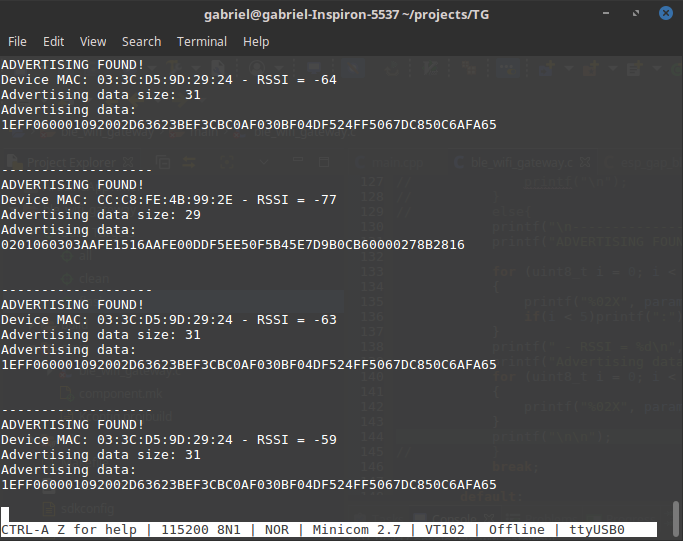
\includegraphics[width=0.8\linewidth]{adv_list.png}
	\captionof{figure}{Pacotes de advertising detectados pelo ESP32}
	\label{fig:adv_list}
\end{center} 

\subsubsection{Filtragem e Decodificação dos pacotes}
Os testes com as funções responsáveis por filtrar e decodificar os pacotes foram
testadas no mesmo modelo, através de mensagens enviadas por meio da porta
serial.

A figura \ref{fig:sesor_decoded_data} mostra os pacotes filtrados
(\dblquote{Packet filtered}) e decodificados(\dblquote{Packet matches}) no
terminal serial, com o endereço do dispositivo e o valor das variáveis medidas.

\begin{center}
	\centering 
	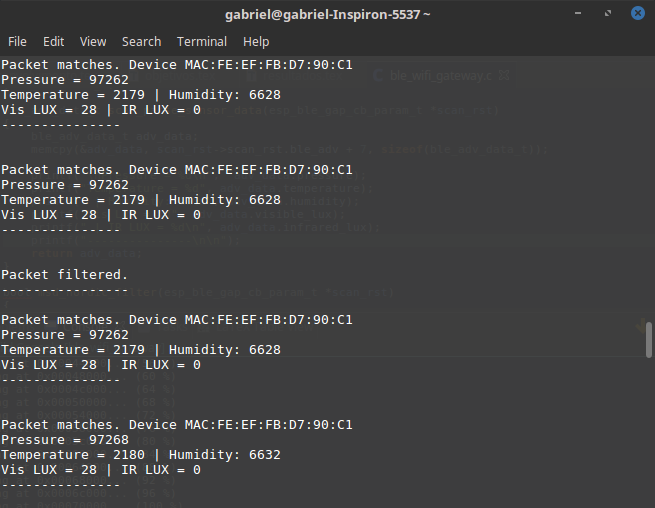
\includegraphics[width=0.8\linewidth]{sesor_decoded_data.png}
	\captionof{figure}{Pacotes de advertising decodificados pelo ESP32}
	\label{fig:sesor_decoded_data}
\end{center} 


\subsubsection{Conexão com o AWS IoT Core}

\subsubsection{Publicação na Internet}

\subsection{Nuvem}

\subsubsection{Comunicação com o Gateway Bluetooth - Wifi}

\subsubsection{Armazenamento}

\subsubsection{Acesso aos dados}

\subsection{Performance energética}

\subsubsection{Medidas de consumo de energia}

\subsubsection{Advertising}

\subsubsection{Conexão Bluetooth}

\subsubsection{Leitura dos sensores}

\subsubsection{Standby}